\documentclass{article}
\usepackage[]{graphicx}
\usepackage[]{fullpage}
\usepackage[]{amsmath}
\usepackage[]{float}
\usepackage[]{siunitx}
\usepackage[]{hyperref}
\usepackage[]{listings}
\hypersetup{
  colorlinks = true,
  linkcolor=blue,
  urlcolor=black,
  citecolor=red
}
\usepackage[toc,page]{appendix}
\title{Optimal Filter Design: The Simplified Real Frequency Technique}
\author{John Rinehart\\ Department of Physics and Astronomy, University of
Waterloo}
\usepackage{color} %red, green, blue, yellow, cyan, magenta, black, white
\definecolor{mygreen}{RGB}{28,172,0} % color values Red, Green, Blue
\definecolor{mylilas}{RGB}{170,55,241}
\begin{document}
\lstset{language=Matlab,%
    %basicstyle=\color{red},
    breaklines=true,%
    morekeywords={matlab2tikz},
    keywordstyle=\color{blue},%
    morekeywords=[2]{1}, keywordstyle=[2]{\color{black}},
    identifierstyle=\color{black},%
    stringstyle=\color{mylilas},
    commentstyle=\color{mygreen},%
    showstringspaces=false,%without this there will be a symbol in the places where there is a space
    numbers=left,%
    numberstyle={\tiny \color{black}},% size of the numbers
    numbersep=9pt, % this defines how far the numbers are from the text
    emph=[1]{for,end,break},emphstyle=[1]\color{red}, %some words to emphasise
    %emph=[2]{word1,word2}, emphstyle=[2]{style},    
}
\maketitle
\tableofcontents
\section*{Introduction}
\addcontentsline{toc}{section}{Motivation}
Filters are an important part of the RF/Microwave signal chain. They can be used
to prevent aliasing of signals used with nonlinear devices (like mixers) and
also to prevent interference from signals with proximal frequency components.
Ever filter is qualified by a number of metrics: insertion loss, rejection,
selectivity, group delay, etc. The topology, number and quality of components
determines the filter's behavior and, as such, must be chosen very carefully.

To add to the filter designer's struggles, it can be shown that it is not
possible to design a filter with arbitrarily large bandwidth and arbitrarily high
gain. The derivation of the gain-bandwidth theorem can be found in reference
\cite{wcd}. Thus, it is up to the designer to push the gain-bandwidth
limits to the limit. This requires high-fidelity components and an optimal
design scheme. Material science and component design is under active research.
This will improve the reliability and performance of the components, themselves.

What is needed, then, is to consider a methodology with which the proper
components for an optimal filter design can be considered. The simplified real
frequency technique (SRFT), devised in 1982 by Herbert Carlin and Binboga Yarman
addresses this problem \cite{srft}. Essentially, the SRFT achieves an optimal
filter design by using computer-aided optimization. This report will describe
SRFT and a MATLAB\textsuperscript{\textregistered} implementation of the SRFT
currently under development. The goal of this report is to demonstrate the
efficacy of the SRFT and a particular microwave design which was implement using
the aformentioned MATLAB\textsuperscript{\textregistered} implementation.

\section*{Theory}
\addcontentsline{toc}{section}{Theory}

The theory behind the SRFT is simple and relies on 4 basic ideas:

\begin{enumerate}
    \item Optimization of Transducer Gain
    \item Kramers-Kronig Relations
    \item The Gewertz Method
    \item Darlington Synthesis (Pole Extraction at Infinity)
\end{enumerate}

\subsection*{Optimization of Transducer Gain}
\addcontentsline{toc}{subsection}{Optimization of Transducer Gain}

The concept of transducer gain optimization is simple: Consider the source and
the load and allow the introduction of some network that maximizes the power
transfer from the source to the lead. This power transfer will be maximum when
the source and the load are conjugately matched. Thus, the problem can be stated
as follows:

\[
\min_{\text{networks}} \left| \left| T_{\text{goal}}(\omega) -
T_{\text{network}}(\omega) \right| \right|
\]

The idea, stated above, is to declare some goal transducer gain function (that may be
physically impossible based on gain-bandwidth considerations). Then, considering
all possible networks, we minimize over the norm of the difference between the
two transducer gain functions. However, we need some way in which to perform
this minimization. So, we next express the transducer gain of the network in
terms of the impedance of the network and the load:

\[ 
T(\omega) = \frac{4 r R}{(x + X)^2 + (r + R)^2} 
\]

Where, above, lower case $r$ and $x$ indicate load quantities and $R$ and $X$
represent network quantities. It should be clear from this description that the
frequency dependence is captured by all of the four circuit quantities: $r, R,
x, X$. It is precisely this frequency dependence that determines the transducer
gain. It should also be noted that the gain appears to be maximized when the
reactance of the load is cancelled by the reactance of the introduced network.
This is a restatement of the conjugate matching principle stated earlier. Now,
for the purposes of this report, the load will always be considered fixed. The
network is introduce in the context of the load and the transducer gain is
maximized.

They way in which SRFT attempts to determine the optimum resistance
characteristic is determined by the relationship between the resistance and
reactance characteristic and will be discussed subsequently.

\subsection*{Kramers-Kronig Relations}
\addcontentsline{toc}{subsection}{Kramers-Kronig Relations}

A really interesting side-effect of having access to a linear, causal system is
that the real and imaginary parts of the transfer function of such a system are
not independent. It can be shown that the relationship between the real and
imaginary parts of a circuit network $R$ and $X$ are as follows (see \cite{wcd}):


\begin{align*}
    R(\omega) &= - \frac{2}{\pi} \int_{0}^{\infty} \frac{\Omega~X(\Omega)}{\Omega^2 -
\omega^2} d\Omega \\
    X(\omega) &= \frac{2\omega}{\pi} \int_{0}^{\infty}
\frac{R(\Omega)}{\Omega^2-\omega^2} d \Omega
\end{align*}

These are known as the Kramers-Kronig relations. It is at this point that the
numerical optimization procedure is introduced.  Imagine that the resistance as
a function of frequency is broken up into many piecewise segments. Then, for
each break frequency $\omega_k$ there exists some resistance $R_k$ at that break
frequency. $R(\omega)$ can now be expressed as:

\[ 
R(\omega) = R_0 + \sum^{n}_{k=1} D_k a_k(\omega) 
\]

where 

\begin{align*}
    a_k(\omega) =&
    \begin{cases}
        1 & \omega \ge \omega_k \\
        \frac{\omega - \omega_{k-1}}{\omega_k - \omega_{k-1}} &\omega_{k-1} \le
        \omega \le \omega_k \\
        0 &\omega < \omega_{k-1}
    \end{cases}
\end{align*}

It is clear from this, then, that $D_k$ represents the slope of the kth break
frequency and, as such:

\[ 
D_k = R_k - R_{k-1} 
\]

If this is the form of $R(\omega)$ that is assumed for the SRFT then it can be
shown that the reactance must be related to $R(\omega)$ by:

\[
X(\omega) = \sum^{n}_{k=1} D_k b_k(\omega)
\]

where
\begin{align*}
    b_k(\omega) = (\pi \left( \omega - \omega_{k-1} \right))^{-1} \big(
&\left( \omega + \omega_k \right) \ln \left| \omega + \omega_k \right| +
\\
&\left( \omega - \omega_k \right) \ln \left| \omega - \omega_k \right| - \\
&\left(\omega + \omega_{k-1} \right) \ln \left| \omega + \omega_{k-1} \right| - 
\\
&\left( \omega - \omega_{k-1} \right) \ln \left| \omega - \omega_{k-1} \right| 
\big)
\end{align*}

This expression for $X(\omega)$ is nothing more than the previous expressions
relating $R(\omega)$ to $X(\omega)$ assuming that $R(\omega)$ has a piecewise
linear form. This piecewise linearity makes it easy to calculate the reactance
on a computer. Since the goal is to reduce the difference between the goal gain
function and the network gain function, the algorithm will perform the
following: It will adjust the $D_k$s using some scheme (gradient ascent, random,
etc.) and will attempt to produce a set of $D_k$s that makes the difference
between $T_{network}$ and $T_{goal}$ a minimum. Those $D_k$s will correspond to
some $R(\omega)$ and some $X(\omega)$. Thus, it would seem that the $D_k$
correspond to some network. It is this point that we have to introduce the way
in which the network is deduced from $R(\omega)$ and $X(\omega)$.

\subsection*{The Gewertz Method}
\addcontentsline{toc}{subsection}{The Gewertz Method}

In order to determine a network from the obtained piecewise linear $R(\omega)$,
I can perform the following. It can be shown that the impedance of the network
and the resistance of the network are related:

\[ 
R(-s^2) = \frac{1}{2} \left( Z(s) + Z(-s) \right) 
\]

where $s = j\omega$. The reason for expression $R$ as a function of $s^2$ is
that the resistance function must be even about $\omega = 0$, by physical
considerations. So, now, consider that the piecewise linear $R(\omega)$ is
approximated by some rational function fit $\tilde{R}(-s^2) =
\frac{p(-s^2)}{q(-s^2)}$.  Now, consider $Z(s) = \frac{n(s)}{d(s)}$, where $n$
and $d$ are the numerator and denominator polynomials of $Z(s)$, respectively.
It can be shown, then, that by relating the coefficients of $p(-s^2)$ with those
of $d(s)$ and $n(s)$ that the following holds (note that $d(s)d(-s) = q(-s^2)$):

\[ 
    \begin{pmatrix} p_0 \\ p_2 \\ \vdots \\ p_{2m} \end{pmatrix} = 
        \begin{pmatrix}
            d_0 & 0    & \ldots & 0 & 0      \\
            d_2 & -d_1 & \ldots & 0 & 0      \\
            \vdots & \vdots & \vdots & \vdots & \vdots \\
            0   &   0  & \ldots & -d_{m-1} & d_{m-2} \\
            0   &   0  & \ldots & 0 & d_{m} 
        \end{pmatrix}
        \begin{pmatrix}
            n_0 \\ n_1 \\ \vdots \\ n_{m-1} \\ n_{m}
        \end{pmatrix}
\]

Above, it is assumed that $p(s) = \sum^{2m-2}_{i=1} p_i s^i$ and similarly with
the other polynomials.

Now, our goal is to solve for $Z(s) = \frac{n(s)}{d(s)}$. We can obtain the
coefficients of $d(s)$ from those of $q(s)$ (we have $q(-s^2)$ from our fit of
$R(-s^2)$) by using spectral factorization. According to \cite{wcd}, any
real non-negative function $A(-s^2)$ can be written as a product, $a_0^2
a(s)a(-s)$, where $a_0$ is real and $a(s)$ is a real monic polynomial. Thus, we
know the coefficients $d_0, d_1, d_2,\ldots, d_{2m}$ which form $d(s)$ since we
know $q(-s^2)$ from having had fit $R(s)$ to a rational function.

We can then invert the above equation to find the numerator polynomial
coefficients. Once we have $n(s)$ from the aforementioned procedure, we form
$Z(s) = \frac{n(s)}{d(s)}$. This is the Gewertz method.

What we need now is a way in which to obtain the network (resistors, inductors,
capacitors) from $Z(s)$. This is what Darlington synthesis enables us to do.

\subsection*{Darlington Synthesis}
\addcontentsline{toc}{subsection}{Darlington Sythesis}

It is shown in reference \cite{wcd} that any realizable impedance function can
be realized as a lossless LC ladder network terminated on a resistor. The proof
will not be given here but a demonstration of the technique will be described.
Assuming that $Z(s)$ is expressed as a rational function (which can always be
done to at least some approximation), then the network can be constructed as
follows:

\[ 
Z(s) = \frac{n_0 + n_1 s + n_2 s^2 + \ldots + n_m s^m}{d_0 + d_1 s + d_2 s^2 +
\ldots + d_m s^m} 
\]

Then, by iterative division, $Z(s)$ can be expressed as a continued fraction:

\[ 
Z(s) = \frac{1}{\frac{d_0 + d_1 s + d_2 s^2 +
\ldots + d_m s^m}{n_0 + n_1 s + n_2 s^2 + \ldots + n_m s^m}} 
\]

Then, using long division, this can be expressed in the form:

\[
Z(s) = \frac{1}{c_0(s) + \frac{1}{c_1(s) + \frac{1}{c_2(s) + \ldots}}}
\]

Now, this is exactly the form of an LC ladder network input impedance. By
construction, $c_0(s)$ is at most a first order polynomial in $s$. This holds
true for other $c_i(s)$ also. Consider the case, for example, when $c_0(s) =
.5s$. This is exactly a capactive admittance of value
\SI[parse-numbers=false]{.5s}{\siemens} which corresponds to a capacitance of
\SI{.5}{\farad}. Thus, the first element in the network would be a shunt
capacitance (since it's an admittance) of \SI{.5}{\farad}. So, apparently,
expressing the impedance in this form by repeating iterative long division is a
way in which the components of the network are made easily visible.

Once the components are identified, all that remains is to simulate the network
determined by the algorithm to ensure that it, indeed, satisfies the properties
desired by the designer; that is, that it approximates well the optimal
gain-bandwidth characteristic.

Now that the theory has been established, a practical example of a filter will
be undertaken and the network will by synthesized and simulated. The
shortcomings of the current implementation will be discussed subsequently.

\section*{Filter Example}
\addcontentsline{toc}{section}{Filter Example}

The following example is taken from section 9.5.2 of reference \cite{opt}. The
load impedance is a series inductor of value \SI{2.3}{\henry}, a shunt capacitor
of value \SI{1.2}{\farad} and a parallel resistor (the load resistance) of value
\SI{1}{\ohm}. Thus, we can express $z(s) = 2.3s + 1/(\frac{1}{1.2s} +
\frac{1}{1})$ (note the lower case usage of z for the load). I have used the
code included in appendix \ref{sec:appendix_a_matlabtextregistered} to generate
the following filter design:

\begin{figure}[H]
    \centering
    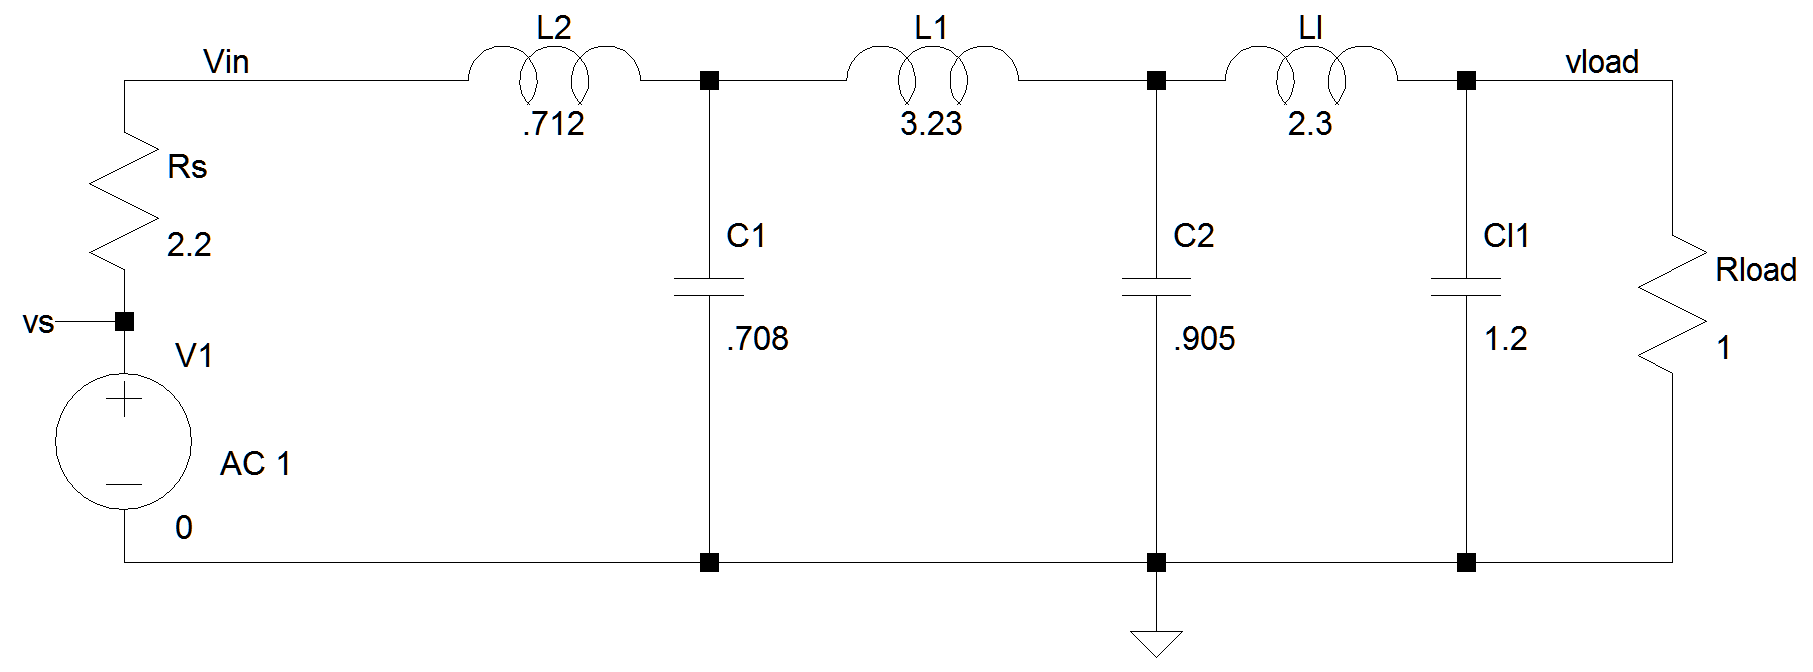
\includegraphics[width=0.8\linewidth]{../img/Load.PNG}
    \caption{Schematic determined by the SRFT}
    \label{fig:load}
\end{figure}

The results of having had simulated this network in
LTSpice\textsuperscript{\textregistered} are given below:

\begin{figure}[H]
    \centering
    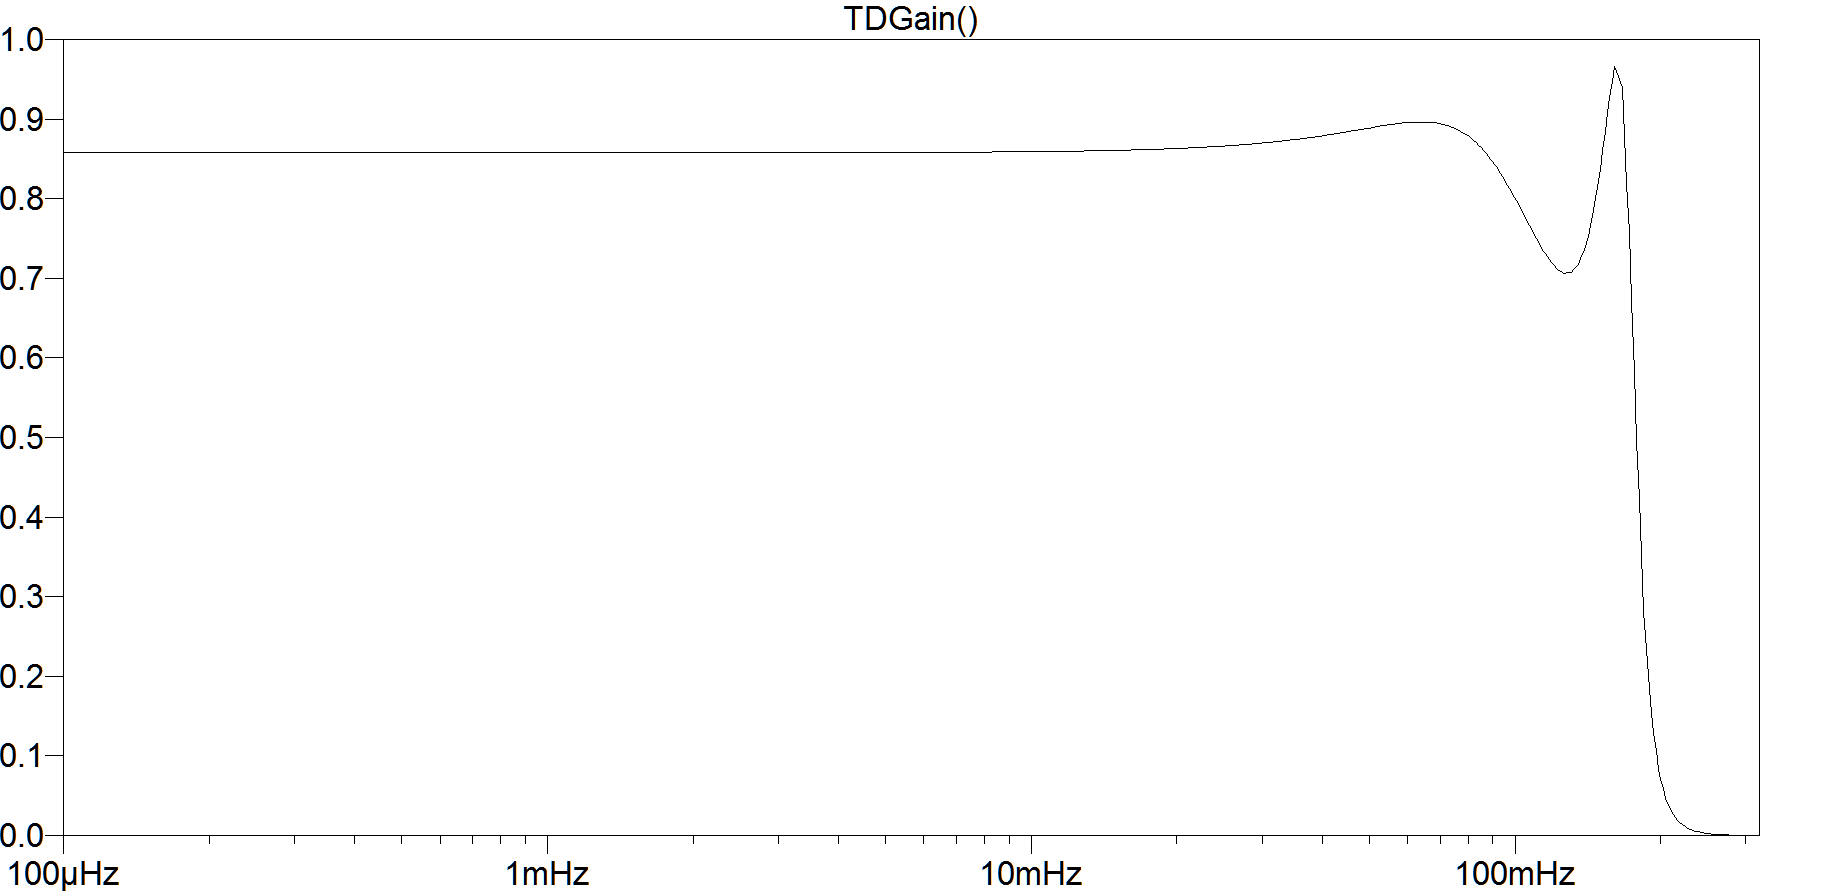
\includegraphics[width=0.8\linewidth]{../img/LTSpiceResults.png}
    \caption{Results of having had simulated the network of figure
    \ref{fig:load} in LTSpice\textsuperscript{\textregistered}}
    \label{fig:LTSpiceResults}
\end{figure}

These component values are currently returned to the
MATLAB\textsuperscript{\textregistered} command line window once the entire SRFT
has been completed. The command line output for this example is shown in the
figure below.

\begin{figure}[H]
    \centering
    \includegraphics[width=0.8\linewidth]{../img/matlabclc.png}
    \caption{Output of the SRFT algorithm in the
    MATLAB\textsuperscript{\textregistered} command line window}
    \label{fig:matlabclc}
\end{figure}
This simulation can be compared to the goal and obtained transducer gain (shown
below):

\begin{figure}[H]
    \centering
    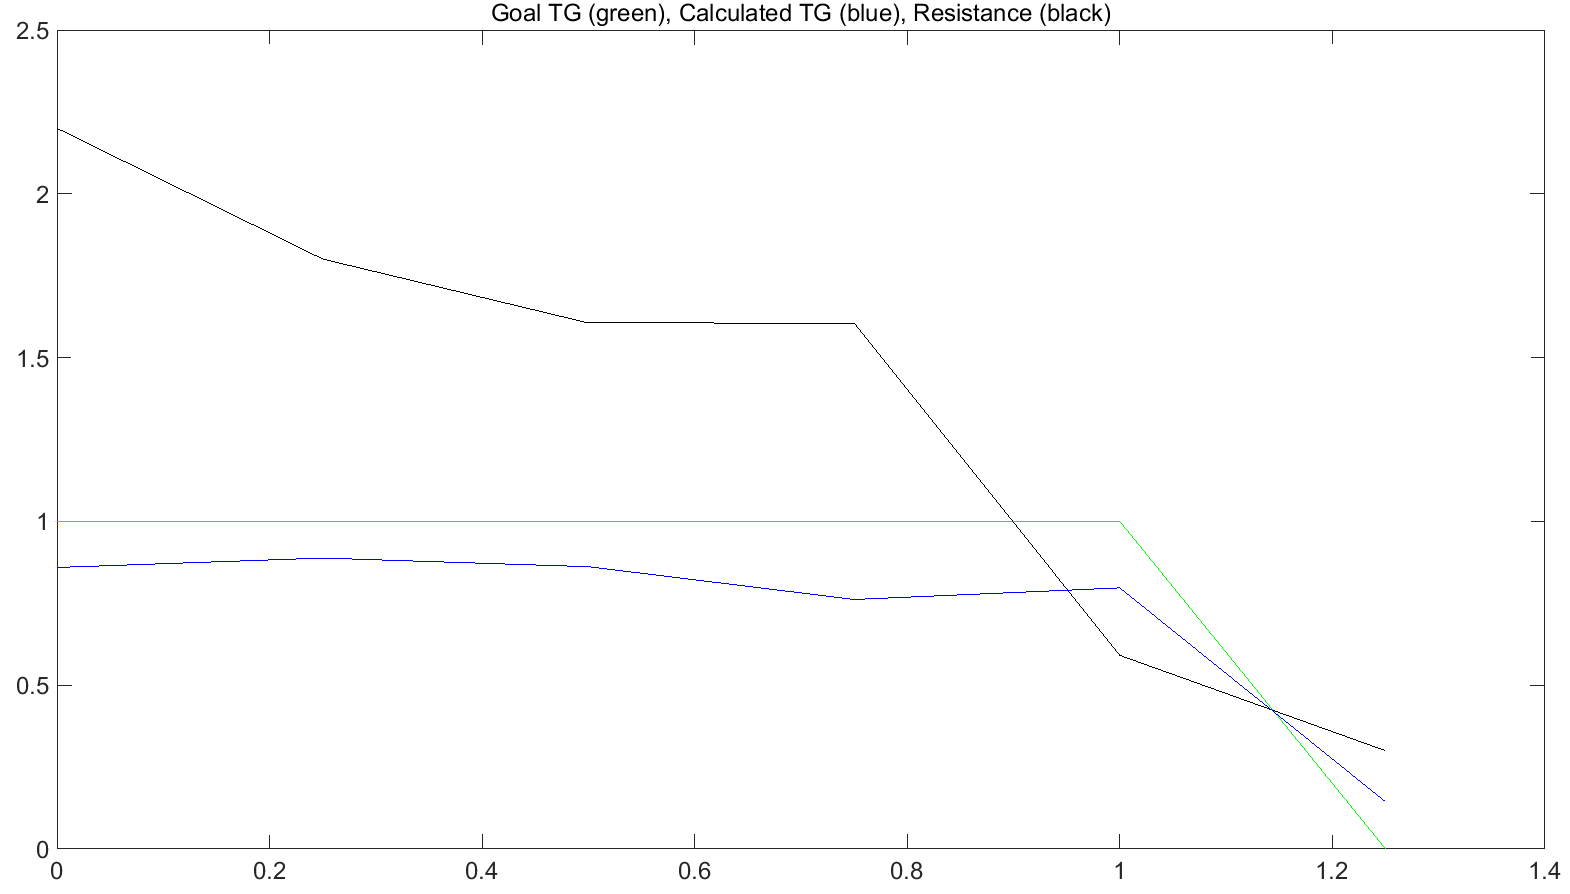
\includegraphics[width=.8\linewidth]{../img/OptimumGain.png}
    \caption{MATLAB\textsuperscript{\textregistered} calculated piecewise
    resistance (black), optimum/goal gain function (green) and numerically-obtained
gain function (blue). The 6 break points ($\omega = 0,.25,.5,.75,1.0,1.25$) are
clearly visible in the piecewise resistance plot. The same vertical axis was
used for both the transducer gain and the resistance plot. The resistance
vertical axis
has units of ohms and the transducer gain is normalized to one (power delivered
to the load is the same as the available power from the source); the horizontal
axis has units of \SI{}{\radian\per\second}}
    \label{fig:../img/OptimumGain}
\end{figure}

The MATLAB\textsuperscript{\textregistered} results were obtained assuming 6
break frequencies. $\omega = 0,.25,.5,.75,1.0,1.25$. There are discrepancies
that exist between the LTSpice\textsuperscript{\textregistered} results and the
MATLAB\textsuperscript{\textregistered} results. There is good reason for this.
One reason is that the MATLAB\textsuperscript{\textregistered} results were
obtained using component values that were precise to within the numerical precision of
the calculations. A more significant reason for the difference, however, is that
the MATLAB\textsuperscript{\textregistered} implementation of the SRFT only
calculates the transducer gain at select points between the break points. The
LTSpice\textsuperscript{\textregistered} results are solved over a more
continuous bandwidth. 

The reason for the seeming discrepancy between the horizontal axes is that the
LTSpice\textsuperscript{\textregistered} results are plotted against linear
frequency (\SI{}{\hertz}) while the MATLAB\textsuperscript{\textregistered}
results are plotted against angular frequency (\SI{}{\radian\per\second}).

So far, no microwave circuit has been designed. However, this topology lends
itself well to design using open stubs on microstrip. All that would be needed
would be to transform the lumped components into transmission line components
using Kuroda's identities (to turn all inductors into capacitors, realizing open
shunt stubs instead of series short stubs) and Richard's transformations to turn
shunt capacitors into open shunt stubs of $\lambda/8$ length (\SI{45}{\degree}).
Time, unfortunately, did not permit for this. The code generation took quite
some time and it is not yet optimal. Future improvements are discussed below.

\section*{Future Work}
\addcontentsline{toc}{section}{Future Work}

There are a number of problems with the code base that was used to replicate the
circuit studied in reference \cite{opt} (this circuit was also used as an example
in \cite{wcd}). The first main problem with the code is the reliance on fmincon
, a MATLAB\textsuperscript{\textregistered} function that is able to solve
nonlinear optimization problems with applied constraints. In this case, the
constraint of decreasing resistance with increasing frequency was applied.

However, nonlinear optimization is subject to the unfortunate problem that
solutions can arise that are not, in general, the best solution. The
optimization procedures, in general, work by determining the best way in which
to ``tweak''/adjust the variables under consideration such as to minimize the
function at hand. The solution relies, then, heavily on the initial conditions
given to the solver. A large improvement to the algorithm would be to express
the problem as that of a linear optimization problem. Then, the sensitivity to
initial conditions is gone and a global minimum is guaranteed.

Next, the Gewertz method that is used in conjunction with Darlington Synthesis
is undesirable. The amount of steps that are undertaken to obtain $Z(s)$ from
$R(-s^2)$ are so many that the chance for numerical or implementation error are
great. A better way to approach the problem would be to obtain $X(s)$ directly
from the piecewise $\tilde{R}(s)$ obtained from the optimization procedure.
Then, once $X(s)$ is known it is easy to construct $Z(s) = R(s) + X(s)$.
Then, a rational function fit of $Z(s)$ can be obtained (to arbitrary numerator
and denominator precision).

Furthermore, this tool, right now, does not accommodate the ``double matching``
problem where both the source and the load are fixed and the best network is to
be obtained. In this tool, the load is fixed and the rest of the network is
allowed to vary.

Finally, a great edition to this tool would be to increase the level of
interactivity and usability. Right now, the script Example9\_2\_1.m uses the
supplied functions in a very particular way that make it easy to adjust the
load, the number of breakpoints, etc. However, it should be possible to ship the
entire SRFT library without the dependence on such a particular script.

In conclusion, numerous researchers have published papers highlighting the feasibility of quantum state tomography using the Wigner representation of the quantum state. However, all of this being said, Wigner state representations have little experimental relevance. Most quantum computational engineers characterize their states using the density matrix representation, which is equivalent. But, considering the case of a quantum system whose states are continuous under the parameter of interest (like coherent states under the parameter $\alpha$) a density matrix representation may not be as direct as a continuous state-space representation as provided by the Wigner function.

Experimentalism aside, though, Wigner functions have been receiving a lot of attention by theoretical physicists within the last decade in that they lend themselves nicely to understanding how much ``quantum resource'' exists in a certain state \cite{Veitch}.  Coherent states of light (the appropriate description of light in the classical regime) are entirely positive in phase space. Fock states, however, must, and are always, negative over portions of the phase space. This motivates correlating the amount of ``quantum resource'' with the amount of negativity of the state's Wigner representation in phase space. So, while the Wigner representation may not be consistently practical to obtain experimentally, it is theoretically useful and is seeing much use in this domain, today (especially in the field of quantum optics).
\begin{appendices}
\section{MATLAB\textsuperscript{\textregistered} Code}
\label{sec:appendix_a_matlabtextregistered}

Below, I have included all of the source code necessary to replicate my results.
The code base is open to many revisions (as discussed in the report). I plan on
making this SRFT project open to the public on Github. This way, SRFT design can
be open to the public.

Nota bene: The code is well-documented. However, there are many blocks that are
commented out that were for testing purposes that can still be used for that
purpose. In my opinion, these blocks do not make reading the source inordinately
difficult.

% Main script file.
\subsection{Example9\_2\_1.m}
The below file is the script file which uses all of the other function files
that are included below.

\lstinputlisting[language=Matlab]{../code/Example9_2_1.m}

\subsection{CheckDecreasing.m}
\lstinputlisting[language=Matlab]{../code/CheckDecreasing.m}

\subsection{ErrorFunction.m}
\lstinputlisting[language=Matlab]{../code/ErrorFunction.m}

\subsection{Gewertz.m}
\lstinputlisting[language=Matlab]{../code/Gewertz.m}

\subsection{PoleExtractionAtInfinity.m}
\lstinputlisting[language=Matlab]{../code/PoleExtractionAtInfinity.m}

\subsection{RsFromDs.m}
\lstinputlisting[language=Matlab]{../code/RsFromDs.m}

\subsection{TransducerGain.m}
\lstinputlisting[language=Matlab]{../code/TransducerGain.m}

\subsection{XsFromDs.m}
\lstinputlisting[language=Matlab]{../code/XsFromDs.m}

\end{appendices}
\bibliographystyle{ieeetr}
\bibliography{Bibliography}
\end{document}
